\documentclass[aps,prd,twocolumn,showpacs,superscriptaddress,groupedaddress,nofootinbib]{revtex4}  % for review and submission
%\documentclass[aps,preprint,showpacs,superscriptaddress,groupedaddress]{revtex4}  % for double-spaced preprint
\usepackage{graphicx}  % needed for figures
\usepackage{dcolumn}   % needed for some tables
\usepackage{bm}        % for math
\usepackage{amsmath,amssymb}   % for math
\usepackage{aas_macros}
\usepackage{multirow}
\usepackage{color}
\usepackage{verbatim}
%\usepackage{times}
\usepackage{url}
\usepackage{hyperref}

% avoids incorrect hyphenation, added Nov/08 by SSR
\hyphenation{ALPGEN}
\hyphenation{EVTGEN}
\hyphenation{PYTHIA}

\newcommand{\mr}{\mathrm}
\newcommand{\tcb}{\textcolor{blue}}
\newcommand{\bea}{\begin{eqnarray}}
\newcommand{\eea}{\end{eqnarray}}
\newcommand{\bmk}{\bm{k}}
\newcommand{\bmx}{\bm{x}}
\newcommand{\la}{\langle}
\newcommand{\ra}{\rangle}
\newcommand{\nl}{\mr{NL}}



\begin{document}
% The following information is for internal review, please remove them for submission
\widetext
% the following line is for submission, including submission to the arXiv!!
%\hspace{5.2in} \mbox{Fermilab-Pub-04/xxx-E}


\title{Reconstruction of Baryon Acoustic Oscillations in 1+1 Dimensions}

%\author{Hong-Ming Zhu}
%\affiliation{Key Laboratory for Computational Astrophysics, National Astronomical Observatories, Chinese Academy of Sciences, 20A Datun Road, Beijing 100012, China}
%\affiliation{University of Chinese Academy of Sciences, Beijing 100049, China}
%
%\author{Ue-Li Pen}
%\affiliation{Canadian Institute for Theoretical Astrophysics, University of Toronto, 60 St. George Street, Toronto, Ontario M5S 3H8, Canada}
%\affiliation{Dunlap Institute for Astronomy and Astrophysics, University of Toronto, 50 St. George Street, Toronto, Ontario M5S 3H4, Canada}
%\affiliation{Canadian Institute for Advanced Research, CIFAR Program in Gravitation and Cosmology, Toronto, Ontario M5G 1Z8, Canada}
%\affiliation{Perimeter Institute for Theoretical Physics, 31 Caroline Street North, Waterloo, Ontario, N2L 2Y5, Canada}
%
%\author{Matthew McQuinn}
%\affiliation{Department of Astronomy, University of Washington, Seattle, WA 98195, USA}
%
%\author{Xuelei Chen}
%\affiliation{Key Laboratory for Computational Astrophysics, National Astronomical Observatories, Chinese Academy of Sciences, 20A Datun Road, Beijing 100012, China}
%\affiliation{University of Chinese Academy of Sciences, Beijing 100049, China}
%\affiliation{Center of High Energy Physics, Peking University, Beijing 100871, China}

\date{\today}

\begin{abstract}
In this paper we introduce a new way to reconstruct BAO peaks in real space.

title 0: Reconstructing the Primordial Density Field in 1+1 Dimensions

title 1: Reconstruction of BAO Peaks in 1+1 Dimensions

title 2: Baryon Acoustic Oscillations Reconstruction in 1+1 Dimensions.

title 2: BAO Reconstruction in 1+1 Dimensions.

\end{abstract}

\pacs{}
\maketitle

%\section{\label{sec:level1}First-level heading}
% sections are not used for PRL papers

{\it Introduction.}---The imprint of baryon acoustic oscillations (BAO) in the
large-scale structure provides a standard ruler to measure the expansion rate
of the Universe. Precise measurements of the BAO feature are crucial for 
probing the dynamics of dark energy.
Nonlinear evolution in the density field damps the oscillations in the linear
power specturm, reducing the BAO signal can be extracted from observations. 
The lost linear BAO information can be partially recovered by the reconstruction
technique []. Precision modelling of the reconstructed density field and 
further improvements of the reconstruction method are of great importance
for measureing the BAO peak at the subpercent level in the current and future
dark energy experiments.

In the standard BAO reconstruction algorithm, the negative Zel'dovich (linear)
displacement is used to reverse the large-scale bulk flows.
The small-scale inhomogeneities in the nonlinear density field is ususally
suppressed using a Gaussian smoothing of scale $R$ so that the smoothed density
field provides a reliable estimation on the linear displacement.
The smoothing scale $R$ should be comparable to the nonlinear scale 
$\sim10\ \mr{Mpc}/h$, where linear approximation breaks down.
Thus, the nonlinear information is not used in the reconstruction. 
However, using smaller smoothing scales in order to include the small-scale 
modes would make the Zel'dovich approximation unvalid and induce
nonlinearities which are difficult to model.
The gain would be huge if these small-scale modes can be exploited, providing
the information about the higher-order displacement field.
The estimated negative Zel'dovich displacement is evaluated at the Eulerian 
position $\bm{x}$ rather than the Lagrangian position $\bm{q}$. The difference
between these two positions is often neglected in the reconstruction, which
is a reasonable first order approximation (See Section 3.1 in Ref. [] for a 
discussion about this). Recently it is suggested that a new correction term
due to this should be included in modelling the displacement (See Appendix A
in Ref.  for more detailed discussions).
In this Letter, we point out that the nonlinear displecement can be solved
from the nonlinear density field and present a new method to reconstruct
the linear BAO information from the nonlinear density field.

The basic idea is to build a curvilinear coordinate system, where the mass per
volume element is constant [3,4]. Consider a numerical grid of coordinates 
$\bm{\xi}\equiv(\xi_1,\ \xi_2,\ \xi_3)$. In order to determine the physical 
position of each lattice point, one needs to specify the Cartesian coordinate 
$\bm{x}(\bm{\xi},\ t)$ of each curvilinear coordinate.
In the Cartesian coordinate system, the metric is just the Kronecker delta
function $\delta_{ij}$, while the curvilinear metric is
\bea
g_{\alpha\beta}=\frac{\partial x^i}{\partial \xi^\alpha}\frac{\partial x^j}{\partial \xi^\beta}\delta_{ij},
\eea
where Latin indices denote Cartesian coordinate labels $x^i$, 
while Greek indices imply curvilinear coordinates $\xi^\alpha$.
As in Refs. [3,4], we define a coordinate transformation that is a pure 
gradient,
\bea
x^i=\xi^\mu\delta^i_\mu+\Delta x^i,
\eea
where
\bea
\Delta x^i\equiv\frac{\partial\phi}{\partial\xi^\nu}\delta^{i\nu}.
\eea
The lattice displacement $\Delta\bm{x}$ is completely determined by the  
potential $\phi$.
The mass density at the curvilinear coordinate $\bm{\xi}$ is 
\bea
\rho(\bm{\xi})=\sqrt{g}\rho(\bm{x}),
\eea
where $\sqrt{g}\equiv\mr{det}(\partial x^i/\partial \xi^\alpha)$ is the volume
element. The potential field $\phi(\bm{\xi})$ which gives $\rho(\bm{\xi})=0$
can be solved using the multigrid alogirthm described in Ref. [].
Since we only have the density field, which is a scalar field, it only allows
us to reconstruct the scaler potential $\phi$ rather than the vector.
The reconstructed density field $\delta_r(\bm{\xi})$ is given by 
\bea
\delta_r(\bm{\xi})=\nabla_{\bm{\xi}}\cdot\Delta\bm{x}(\bm{\xi}).
\eea

In the Lagrangian approach to the nonlinear structure formation, 
the displacement field $\bm{\Psi}(\bm{q},\tau)$ fully describes the motion of
the mass elements.
The Eulerian position $\bm{x}$ of a mass element is
\bea
\bm{x}=\bm{q}+\bm{\Psi}(\bm{q},\tau),
\eea
where $\bm{q}$ is the initial Lagrangian position of this mass element.
The displacement field $\bm{\Psi}$ can be decomposed into an irrotational part
and a curl part,
\bea
\bm{\Psi}=\bm{\Psi}_E+\bm{\Psi}_B,
\eea
where $\nabla\times\bm{\Psi}_E=0$ and $\nabla\cdot\bm{\Psi}_B=0$.
In the case that particles describe an irrotational potential flow, 
$\bm{\Psi}_E$ fully describes the motion of the mass elements.
In reality, shell crossing happens in the nonlinear regime, and the emergence
of vorticity leads to the growth of $\bm{\Psi}_B$. 
The reconstructed lattice displacement $\Delta\bm{x}$ describes the nonlinear
motion beyond the Zel'dovich displacement.


The real displacement field is available in $N$-body simulations. It can be
decomposed and compared with the reconstructed lattice displacement to see
how much information is reconstructed. 
\tcb{I think this is what Qiaoyin and Haoran working on now?}
%=======================================


{\it Reconstruction algorithm.}---The Lagrangian displacement can be solved
easily in 1+1 dimensions by ordering of the mass elements.

(1) Solve the displacement $\Psi(q)$ field by ordering of the mass elements.

(2) Take the differential derivative of $\Psi(q)$ to get the reconstructed
density field $\delta_r(\bm{q})=-\nabla_{\bm{q}}\Psi(\bm{q})$.
$\delta_r(\bm{q})=-\partial\Psi(q)/\partial q$.

To solve the displacement field, we combine grids to get two fields with
five PM elements per grid and ten PM elements per grid, respectively.

Reconstruction from the gridded density field can be implemented following
the same principle, which we adopt here [].
%=======================================


{\it Simulations.}---We adopt the 1D $N$-body simualtions in 
Ref. \cite{2016matt}
and use outputs at $z=0$. The simulation box is $10^8\ \mr{Mpc}$ with 
$3\times10^8$ grids and $3\times10^8$ PM elements.
We scale the intial density field by the linear
growth factor to get the linear density field $\delta_L$ at $z=0$. 
Note that $\delta_L$ has been rescaled using the linear growth function
to the same redshift as $\delta$. 


Figure \ref{fig:ps} shows the linear, nonlinear and reconstructed power spectra,
as well as the cross-corrlation power spectra.
The correlation of the reconstruction density field $\delta_r$ with the linear
density field $\delta_L$ is much better than that of the raw nonlinear density 
field $\delta$. The wiggles in the reconstructed power spectrum are also much 
more transparent than the raw nonlinear power spectrum.

\begin{figure}[tbp]
\begin{center}
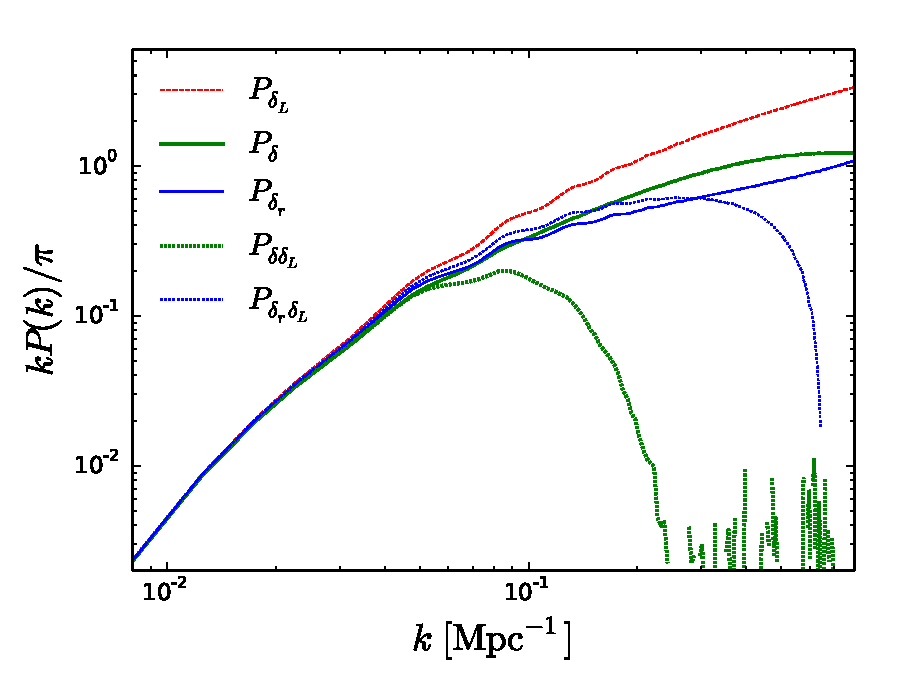
\includegraphics[width=0.48\textwidth]{f3x.eps}
\end{center}
\vspace{-0.7cm}
\caption{The power spectra of the linear (dashed line), nonlinear (thick solid
line), and reconstructed (thin solid line) fields. 
We also plot the nonlinear-linear (thick dotted line) and 
reconstructed-linear (thin dotted line) cross-correlation power spectra.}
\label{fig:ps}
\end{figure}
%=======================================


{\it Results.}---To convenienty quantify the linear information $\delta_L$ in 
the nonlinear density field $\delta$, we decompose the nonlinear density field
$\delta$ as
\begin{eqnarray}
\delta(\bm{k})=b(\bm{k})\delta_L(\bm{k})+\delta_N(\bm{k}).
\end{eqnarray}
Here, $b\delta_L$ is completely correlated with the linear density field 
$\delta_L$ and $b=P_{\delta\delta_L}/P_{\delta_L}$.
Nonlinear evolution drives $b$ to drop from unity, reducing the linear signal.
$\delta_N$ is generated in the nonlinear evolution and thus uncorrelated with
the linear density field $\delta_L$, further reducing $b\delta_L$ with respect
to $\delta$. This part induces noises in the measurement of BAO. 
Hence we denote it with a subscript ``$N$''. 
Such decomposition helps to write the nonlinear power spectrum as
\bea
P_\delta(k)=\mathcal{D}(k)P_{\delta_L}(k)+P_{\delta_N}(k),
\eea
where $\mathcal{D}=b^2$ describes the damping of the linear power specturm.
The reconstructed power spectrum $P_{\delta_r}$ can be describe in the same way.
Here, $b(\bm{k})$ is often referred as the ``propagator'' 
and $n(\bm{k})$ is usually
called the mode-coupling term \cite{2006crocce,2008crocce,2008matsubara}.
\tcb{still to be modified}

\begin{figure}[tbp]
\begin{center}
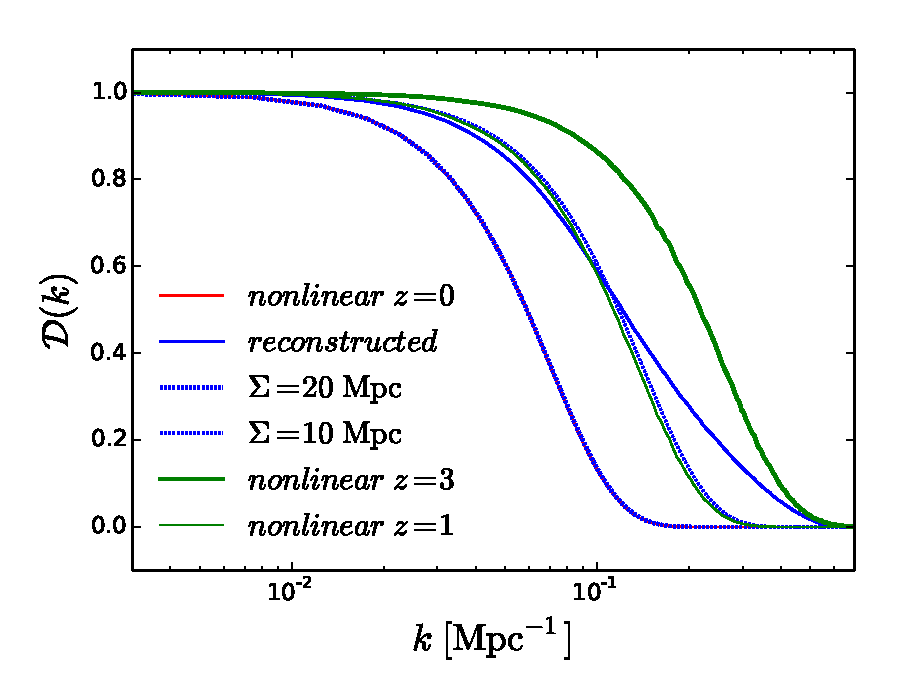
\includegraphics[width=0.48\textwidth]{f6x.eps}
\end{center}
\vspace{-0.7cm}
\caption{The damping factors for the nonlinear (thin solid line) and 
reconstructed (thick solid line) fields. The Gaussian BAO damping models with 
$\Sigma=20\ \mr{Mpc}$ (thick dotted line) and $\Sigma=10\ \mr{Mpc}$ (thin dotted
line).}
\label{fig:damp}
\end{figure}

Figure \ref{fig:damp} shows the damping functions for the raw and reconstructed 
fields. The nonlinear damping of the linear power spectrum is 
significantly reduced after reconstruction. We also overplot the best-fitting 
Gaussian BAO damping model,
\bea
\mathcal{D}(k)=\mr{e}^{-k^2\Sigma^2/2},
\eea
with $\Sigma=?\ \mr{Mpc}$ and $?\ \mr{Mpc}$ for the nonlinear and reconstructed 
fields. The new BAO reconstruction algorithm reduces the the nonlinear damping
scale $\Sigma$ by ?? per cent, i.e., a of ??. The damping factor is above 0.9
for $k\lesssim?\ \mr{Mpc}^{-1}$ indicating (almost) perfect reconstruction. 
\tcb{how to best quantify the reduction of damping? }
However, the 100 per cent reconstruction, cancelling any nonlinear effects,
is still unachievable, as some information has been irreversibly lost. (more 
discissions)

\begin{figure}[tbp]
\begin{center}
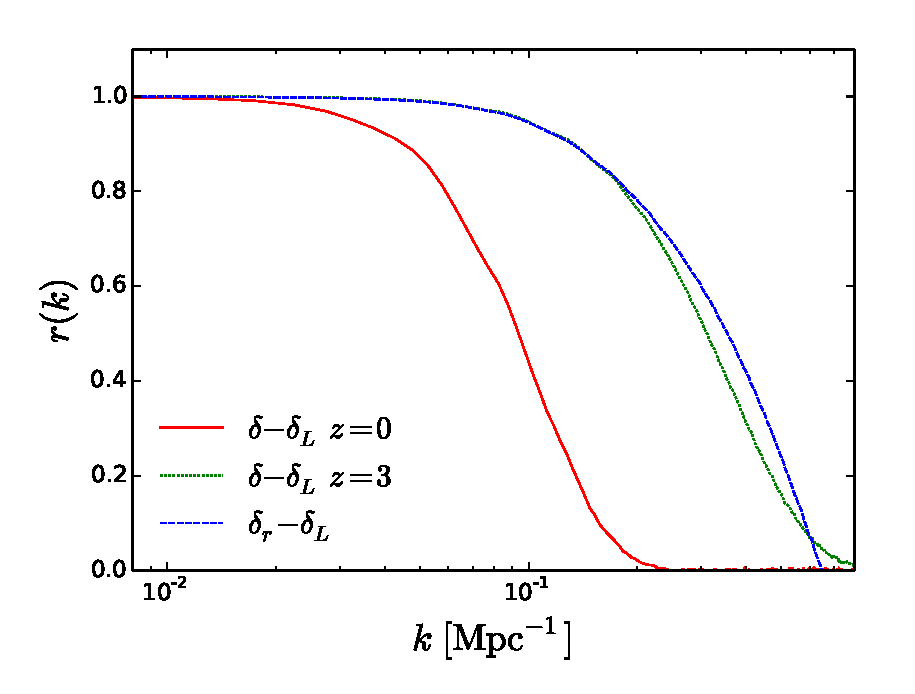
\includegraphics[width=0.48\textwidth]{f7x.eps}
\end{center}
\vspace{-0.7cm}
\caption{The $\delta-\delta_L$ correlation coefficients at $z=0$ (solid
line) and $z=3$ (dotted line), as well as the $\delta_r-\delta_L$ 
correlation coefficient (dashed line).}
\label{fig:xcc}
\end{figure}

Reconstruction also reduces the noise term $P_{\delta_N}$. To demonstrate this,
in Fig. \ref{fig:xcc} we plot the  cross-correltion coefficient 
\bea
r(k)=\frac{P_{\delta\delta_L}(k)}
{\sqrt{P_{\delta}(k)P_{\delta_L}(k)}}
=\frac{1}{\sqrt{1+\eta(k)}},
\eea
where $\eta=P_n/(\mathcal{D}P_{\delta_L})$ quantifies the relative amplitude
of $\delta_N$ with respect to $b\delta_L$. The correlation of $\delta_r$ with
$\delta_L$ is as good as that of $\delta$ at $z=3$.
\tcb{how to quantify this better?}

Distribution functions 
\begin{figure}[tbp]
\begin{center}
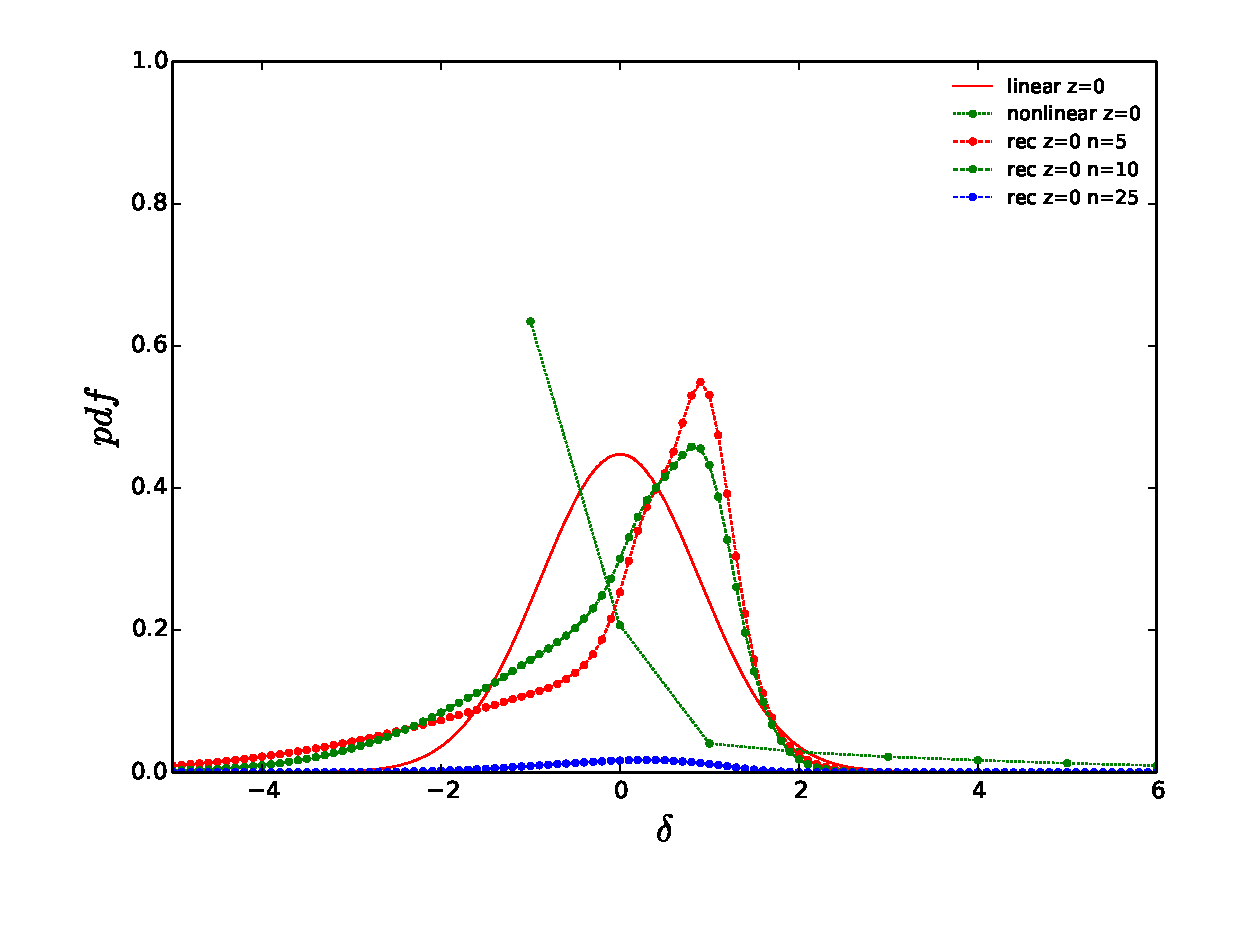
\includegraphics[width=0.48\textwidth]{f9.eps}
\end{center}
\vspace{-0.7cm}
\caption{The distribution functions.}
\label{fig:pdf}
\end{figure}


%=======================================


{\it Discussions.}---The new method significantly
improves the expansion rate measurement from BAO. (more discussions?) 


This method can be generalized to the 3D case. 
We leave this
to future work.



Comparision with and Implications for the standard BAO reconstruction: exact 
Lagrangian displacement,
nonlinear displacement, which is easier to model.

If use the displacement solved in this paper for the standard BAO rec, we expect
the performance will become much better but still not as good as our results.
%=======================================


We acknowledge the support of the Chinese MoST 863 program under Grant 
No. 2012AA121701, the CAS Science Strategic Priority Research Program 
XDB09000000, the NSFC under Grant No. 11373030, IAS at Tsinghua University, 
 and NSERC.
The Dunlap Institute is funded through an endowment established by the David Dunlap family and the University of Toronto.
Research at the Perimeter Institute is supported by the Government of Canada
through Industry Canada and by the Province of Ontario through the Ministry of
Research $\&$ Innovation.

\bibliographystyle{apsrev}
\bibliography{1d}

\end{document}
